\documentclass{article}
\usepackage{fancyhdr}
\pagestyle{fancy}
\fancyfoot{}
\fancyfoot[C]{\thepage}
\rhead{Yarosevich - 1064712}
\usepackage{setspace}
\usepackage{siunitx} % Provides the \SI{}{} and \si{} command for typesetting SI units
\usepackage{graphicx} % Required for the inclusion of images
\usepackage{amsmath} % Required for some math elements 
\usepackage[export]{adjustbox} % loads also graphicx
\usepackage{listings}
\usepackage{setspace}
\usepackage{matlab-prettifier}
\usepackage{float}
\usepackage[most]{tcolorbox}
\usepackage{amsfonts}
\usepackage{color}
\usepackage{physics}
\usepackage{titlesec}
\usepackage{caption}
\usepackage{subcaption}
\usepackage{python}
\usepackage{placeins}
\usepackage{bm}
\usepackage{esvect}
\newcommand{\uveci}{{\bm{\hat{\textnormal{\bfseries\i}}}}}
\newcommand{\uvecj}{{\bm{\hat{\textnormal{\bfseries\j}}}}}
\DeclareRobustCommand{\uvec}[1]{{%
  \ifcsname uvec#1\endcsname
     \csname uvec#1\endcsname
   \else
    \bm{\hat{\mathbf{#1}}}%
   \fi
}}
\lstset{
  basicstyle=\ttfamily,
  columns=fullflexible,
  frame=single,
  breaklines=true,
  postbreak=\mbox{\textcolor{red}{$\hookrightarrow$}\space},
}


\newcommand{\R}{\mathbb{R}}

\usepackage{xcolor}

\DeclareCaptionFont{white}{\color{white}}
\DeclareCaptionFormat{listing}{%
  \parbox{\textwidth}{\colorbox{gray}{\parbox{\textwidth}{#1#2#3}}\vskip-4pt}}
\captionsetup[lstlisting]{format=listing,labelfont=white,textfont=white}
\lstset{frame=lrb,xleftmargin=\fboxsep,xrightmargin=-\fboxsep}
\titleformat{\section}[runin]
  {\normalfont\Large\bfseries}{\thesection}{1em}{}
\titleformat{\subsection}[runin]
  {\normalfont\large\bfseries}{\thesubsection}{1em}{}


\setlength\parindent{0pt} % Removes all indentation from paragraphs

\renewcommand{\labelenumi}{\alph{enumi}.} % Make numbering in the enumerate environment by letter rather than number (e.g. section 6)

%\usepackage{times} % Uncomment to use the Times New Roman font

%----------------------------------------------------------------------------------------
%	DOCUMENT INFORMATION
%----------------------------------------------------------------------------------------

\title{AMATH 522: Homework 2 \\Due October, 28 2019 \\ ID: 1064712} % Title

\author{Trent \textsc{Yarosevich}} % Author name

\date{\today} % Date for the report

\begin{document}
\maketitle % Insert the title, author and date
\setlength\parindent{1cm}

\begin{center}
\begin{tabular}{l r}
%Date Performed: December 1, 2017 \\ % Date the experiment was performed
Instructor: Professor Eric Shea-Brown % Instructor/supervisor
\end{tabular}
\end{center}
\doublespacing
% If you wish to include an abstract, uncomment the lines below
% \begin{abstract}
% Abstract text
% \end{abstract}

%----------------------------------------------------------------------------------------
%	SECTION 1
%----------------------------------------------------------------------------------------
\section*{\textbf{(II)}}
Similarly to the scenario of a channel with a single open state, we have four different ways the channel can be open, and thus four different ways we can have a 'dwell', that is to say, the channel remaining in any of these four open states for a period of time.\\
\\
If we imagine a Markov Transition matrix, each of these states will have a probability $a_{jj}$ of remaining in its current state. Suppose we have a random variable $X(x)$ representing the state of the channel $S_j$ and $k$ is some time increment. Then $P(X(k) = S_j$ is the probability $X$ is in some particular state at some particular time. It follows that $P(X(k+1) = S_J$ is the probability it is still in this state at the next time step. This would be the probability $a_{jj}$ from the Markov Transition matrix, so we have $P(x(k+1) = S_j) = a_{jj}$. At each step $k+m$ we thus have $P(X(k+m) = S_j) = a_{jj}^{m-1}$. Lastly if we are to know that a dwell time has occurred and finished, we must also take into account the channel transitioning away from the state it was in, which means multiplying the above probability by the $1-a_{jj}$, or the probability that $S_j$ transitions to another state. \\
\\
Now, since this ion channel has four open states, the Markov Transition matrix will have four probabilities associated with the channel staying in a given open state for $m$ time steps. Let's call these $S_{1,2,3,4}$ and $a_{11,22,33,44}$. The probability that the channel will remain open and in the same open state for a given time $m$ is thus the sum of each of these dwell probabilities:
\begin{equation}
\begin{aligned}
P(X(k+m) = S_{open}) = a_{11}^{m-1}(1-a_{11})+ a_{22}^{m-1}(1-a_{22})+ a_{33}^{m-1}(1-a_{33})+ a_{44}^{m-1}(1-a_{44})
 \end{aligned}
\end{equation}
Or written a little differently to represent the distribution of a dwell time $k$:
\begin{equation}
\begin{aligned}
P(m = k) = a_{11}^{k-1}(1-a_{11})+ a_{22}^{k-1}(1-a_{22})+ a_{33}^{k-1}(1-a_{33})+ a_{44}^{k-1}(1-a_{44})
 \end{aligned}
\end{equation}
This distribution is exponential since each term in the sum is some constant $\frac{1-a_{jj}}{a_{jj}}$ multiplied by an exponential, which we can call $\lambda^k$ in accordance with how we wrote it in class. Thus we have a sum of four exponentials representing the distribution of dwell times $m$.

\section*{\textbf{(III)}}
Below is the histogram plot of data from a simulation using Python. The simulation used 1,000,000 realizations of the channel, and then iterates over a list of states numbered 0 through 3 counting how long the simulation dwelt in each state. The result is then plotted as a histogram with a logarithmic scale on the $x$ axis, which clearly shows that first order polynomial fit is not sufficient, and indeed as expected a second-order polynomial fit would probably suffice, on account of the two exponentials. 

\begin{center}
    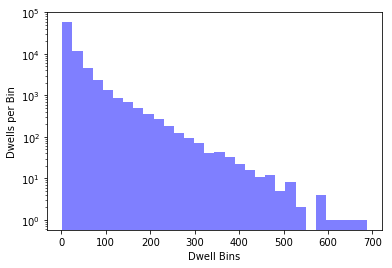
\includegraphics[scale = .75]{hw2_part3_2.png}
    %\captionof{figure}{D}
    %\label{fig: D}
\end{center}
\begin{lstlisting}[language = Python]
#%%
import numpy as np
import matplotlib.pyplot as plt
import random as rd

numsteps = 2000000
dwell_list = []
A = np.array([[.98, .1, 0], [.02, .7, .05], [0, .2, .95]])
states = np.zeros(numsteps, dtype = 'int')
states[0] = 0

# Realizations of the channel as it transitions. 
Note I later learned how to do this more efficiently,
# but this was how I did it the first time.
for k in np.arange(0, numsteps - 1):
    if states[k] == 0:
        states[k+1] = np.random.choice(3, 1, p = [.98, .02, 0])
    if states[k] == 1:
        states[k+1] = np.random.choice(3, 1, p = [.1, .7, .2])
    if states[k] == 2:
        states[k+1] = np.random.choice(3, 1, p = [0, .05, .95])

# Reduces the closed states to zero and the open states to 1.
reduced_states = states[:]
for i in range(0, len(reduced_states)):
    if reduced_states[i] == 1:
        reduced_states[i] = 0
for i in range(0, len(reduced_states)):
    if reduced_states[i] == 2:
        reduced_states[i] = 1

last_dwell = 0
count = 1

# Counts the length of each dwell and stores.
for i in range(1, len(reduced_states)):
    if reduced_states[i] != reduced_states[i-1]:
        dwell_list.append(count)
        count = 1
    count = count +1

 n_bins = 30
n, bins, patches = plt.hist(dwell_list, n_bins, facecolor='blue', alpha=0.5)
plt.yscale('log')
plt.xlabel('Dwell Bins')
plt.ylabel('Dwells per Bin')
plt.show()
\end{lstlisting}

\section*{\textbf{(IV)}}
Below are figures of simulations that used a large number of realizations of the ion channels at equilibrium in order to simulate the probability distribution of spikes for given threshholds. I was a little confused based on what I saw when I plotted these probabilities and so I checked the scaling of the mean charge and variance, which yielded results in line with what we learned in class, namely that as the number of channels increases, the signal to noise ratio should improve. These were just from a few randomly chosen sims, but the numbers were as follows:\\
\\
With $N_{in} = 100$ and $N_{out} = 50$:\\
Mean net current: 10.028\\
Variance of net current: 36.083216\\
SNR = 1.666\\
\\
With $N_{in} = 10$ and $N_{out} = 5$:\\
Mean net current: 1.016\\
Var of net current: 3.813\\
SNR = .5212\\
\\
With $N_{in} = 1000$ and $N_{out}$ = 500:\\
Mean net current: 99.45\\
Variance of net current: 361.38\\
SNR = 5.2315\\
\\
Based on this information it seems the signal to noise ratio was inded increasing. Given that there is a note in the handwritten notes that the distribution should start to become determinate on \textit{a scale of the mean current}, I tried plotting the different $N$ counts with scaling of the threshhold relative to the mean current. This produced the kind of result I had expected, namely that as the plot passes a certain threshhold where the Neuron is going to become unlikely to fire, the transition happens very quickly. Whether or not this is correct, or if there is actually some problem with my simulation, I am not sure. Below are the three plots: sorry for the lack of labels, something is up with my latex package and I don't have time to figure it out.\\
\\
\begin{center}
    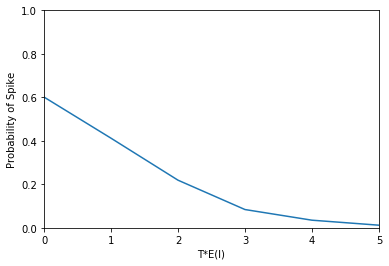
\includegraphics[scale = .6]{part4_10_5.png}
    %\captionof{$N_{in} = 10$, $N_{out} = 5$}{D}
    \label{Bla?}
        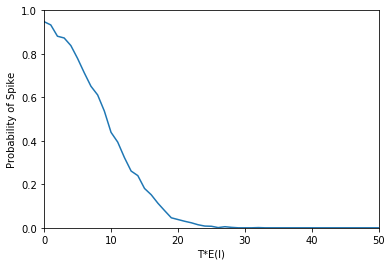
\includegraphics[scale = .6]{part4_100_50.png}
    %\captionof{$N_{in} = 100$, $N_{out} = 50$}{D}
    %\label{fig: D}
        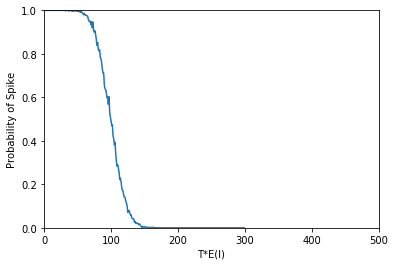
\includegraphics[scale = .6]{part4_1000_500.png}
    %\captionof{$N_{in} = 1000$, $N_{out} = 500$}{D}
    %\label{fig: D}
\end{center}

Mathematically, this approach to determinacy on the scale of the mean is occurring because the ratio of the net charge compared to the standard deviation of the net charge increases as the number of channels increases.

Since I didn't see any deeper mathematical explanation than this, which could simply be a failure on my part, I dipped my toes into some literature on the subject. After glancing at a few papers, I found one that was quite illuminating as to how relevant this question of spiking determinacy is to current neuroscience. White, Rubenstein and Kay provide a nice overview in "Channel noice in neurons" (citation below) of how the notion that spiking threshholds are deterministic with larger numbers of channels is not entirely true (131-132). Indeed, citing a very familiar looking figure of the probability of neurons with three different channel counts spiking, we see a very similar gradation to the probability distribution as shown in the figures from my simulation (assuming using the mean scaling is correct and I didn't inadvertently massage my data). They also reference other research that actually quantifies this gradation (132) Below is the figure in question:
\begin{center}
    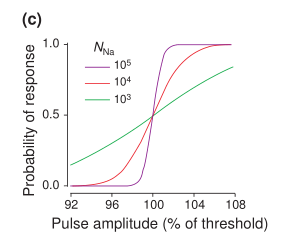
\includegraphics[scale = 1]{paper_figure.png}
    %\captionof{figure}{D}
    %\label{fig: D}
\end{center}

Insofar as building reliable neurons, it would seem that some gradation to this distribution is acceptable and still allows for a reliable function. Quite interestingly, the authors speculate there could be an adaptive factor in the evolution of these differing channel counts, and that due to the considerable oxygen demands of very high channel count neurons, some "anoxia-tolerant animals use reduced channel numbers in order to keep oxygen demand low." (135) I personally found this very fascinating as it is another example of how evolution can optimize the most subtle metabolic function for particular environments.\\
\\
Below are the code for Part 4 and a citation for the paper.

\begin{lstlisting}[language = Python]
#%%
# Part 4.)
import numpy as np
import matplotlib.pyplot as plt
import random as rd


N_in = 1000
N_out = 500
p_in = .4
p_out = .6
numsteps = 1000
T = np.arange(300)
p_T = np.zeros(len(T))
current_list = np.zeros(numsteps)
mean = N_in*p_in - N_out*p_out

# Simulate realizations compared against each threshhold T
for k in np.arange(0, len(T)):
    spike = 0.0
    
    # Simulate lots of realizations of N
    for i in np.arange(0, numsteps):
        # Generates a coin toss vector for the inward and outward channels
        # in which 'open' corresponds to 1. Sums the vector to ascertain
        # the number of open channels in a realization.
        N_in_open = np.sum(np.random.choice([1, 0], size = N_in, p = [p_in, 1 - p_in]))
        N_out_open = np.sum(np.random.choice([1,0], size = N_out, p = [p_out, 1 - p_out]))
        # The net current, open inward channels minus open outward.
        net_current = N_in_open - N_out_open
        # IF the net current is more than T, a spike occurs
        if net_current > k:
            spike = spike + 1.0
        if k == 1:
            current_list[i] = net_current
            
    # Once numsteps realizations have been simulated, divides the number
    # of spikes by the total number of realizations to get the probability
    # that a spike will occur with a given threshhold T
    p_T[k] = spike/numsteps

plt.figure(1)
plt.plot(T, p_T)
plt.xlabel('T*E(I)')
plt.ylabel('Probability of Spike')
plt.axis([0, 5*mean, 0, 1])

plt.show()
\end{lstlisting}
\underline{Works Cited}\\
\\
White, John A, et al. “Channel Noise in Neurons.” Trends in Neurosciences, vol. 23, no. 3, 2000, pp. 131–137.

\end{document}